\chapter{機率與機率分布}
    利用敘述性統計了解資料的分布後,我們就準備要步入推論性統計的範疇了。推論性統計的內涵是將資料抽樣的不確定性以系統性的方式納入考量後,給出資料隱含的結論,因此在進入推論性統計之前,我們必須先熟悉量化抽樣不確定性的數學工具-機率。在這一章,我們會先複習機率以及條件機率的定義,並說明由條件機率衍生出的貝氏定理與其實際應用。然後,我們會介紹隨機變數的概念、常見的隨機變數分布、以及這些分布的特性。本章會開始出現較多的數學符號,但大部分都只牽涉加減乘除,只有一小部分會需要用到積分符號。
    
    \begin{introduction}[第 \thechapter 章學習目標]
        \item 了解機率以及條件機率的意義
        \item 了解貝氏定理以及其於流行病學上的應用
        \item 常見的離散型與連續型分布以及其特性
    \end{introduction}

\section{基礎機率}
\subsection{機率的定義}
    \textit{機率}(probability)又稱或然率或是概率,用來度量一個事件發生可能性,定義為介於 0 和 1 之間的實數。機率越接近 1,代表事件發生的可能性越高,而機率等於 1 代表事件必然發生;反之,機率越接近 0,代表事件發生的可能性越低,而機率等於 0 代表事件不可能發生。對於機率的解釋,一般可以分成兩大流派:\textit{客觀機率}(objective probability)和\textit{主觀機率}(subjective probability)。其中客觀機率又可以分成兩種定義方式:\textit{古典機率} (classical probability) 和\textit{頻率機率} (frequentist probability)。我們可以用「擲兩個骰子得到之總點數為 3 的機率」來說明這三種機率定義方式:
    \begin{itemize}
        \item \textbf{古典機率}:古典機率是最原始的機率定義方法,此定義可以追溯到18世紀的數學家拉普拉斯(Pierre-Simon Laplace)。古典機率認為,首先要找到一群發生可能性均相同的簡單事件(simple events),例如有 $n$ 個這樣的簡單事件。然後,我們可以將我們有興趣的事件分解為 $k$ 個簡單事件的組合。這樣一來,我們有興趣的事件的發生機率就是 $k/n$。例如,擲兩個骰子後,將第一個骰子的點數 a 和第二個骰子的點數 b 記為 (a,b),就可以建構出 36 種可能性相同的簡單事件:(1,1), (1,2), (1,3), ... (1,6), (2,1), (2,2), ..., (6,6)。而我們有興趣的事件「得到總點數為 3」可以分解為兩種簡單事件 (1,2) 和 (2,1),所以「擲兩個骰子得到之總點數為 3 的機率」等於 $2/36 = 1/18$。這種定義雖然簡單直觀,但有兩個主要缺點:首先,「可能性均相同的簡單事件」含有「可能性」在裡面,所以這種定義方法有自己指涉自己的套套邏輯之嫌;另外,符合定義的簡單事件不見得存在,例如在上述的例子中,如果骰子是灌鉛的骰子,那麼就找不到可能性相同的簡單事件了。
        \item \textbf{頻率機率}:頻率機率認為,要探討事件的機率,首先必須要有可重複的隨機試驗,例如我們這裡的隨機試驗就是丟兩顆骰子並記錄點數。該隨機試驗的所有可能結果所組成的集合叫做\textit{樣本空間}(sample space),通常記為$\Omega$,因此例子中的樣本空間就是 36 種可能點數組合的集合,也就是 $\Omega = \{(1,1), (1,2), (1,3), ... (1,6), (2,1), (2,2), ..., (6,6)\}$。注意到這裡我們並未要求樣本空間中所有結果的可能性相等,因此和古典機率不同。\textit{事件}(event)就是樣本空間的子集合,例子中「得到總點數為 3」的事件即對應到 $A = \{(1,2),(2,1)\}$ 這個子集合。重複該試驗多次以後,事件發生的次數 $k$ 和試驗次數 $n$ 的比值雖可能不固定,但是隨著試驗次數增多終將會趨近一個數值,而該數值就是事件發生的機率。頻率機率的定義解決了古典機率的兩大缺點,但其奠基於「可重複隨機試驗」的事實也引起批評:如果我們關心的事件不可能重複試驗,例如「明天台北發生地震」、「某國總統被成功彈劾」或「某病患將在 24 小時內離開加護病房」,那麼頻率機率的定義就顯得不合適。
        \item \textbf{主觀機率}:主觀機率認為機率是個人信念的一種度量,因此「擲兩個骰子得到之總點數為 3 的機率」是我們基於已知的事實(例如骰子的製作過程、投擲的隨機性)評估出擲出骰子後總點數為 3 的可能性。和頻率機率的差異在於,頻率機率認為存在可重複的隨機試驗,該試驗的條件可能未知,但已固定。主觀機率則認爲針對試驗的方方面面的不確定性和主觀認知,都應該納入機率考量。因此不同人針對同一事件的主觀機率,也會隨著每個人的信念和經驗而不同。
    \end{itemize}
    在後續的課程中,大部分時候我們選擇的機率定義為頻率機率,但必要的時候,我們也會改用主觀機率以方便實務上的解釋。讀者閱讀時也不妨想想各處提到的機率是用哪種方式定義比較合適。
\subsection{機率的基本性質}
    在頻率機率的定義下,假設樣本空間是 $\Omega$,而 $A$, $B$ 代表任意的事件,我們定義如下:
    \begin{itemize}
        \item $\PP(A)$ 代表 $A$ 事件發生的機率。
        \item $\bar{A} = \Omega \backslash A$ 為 $A$ 的\textit{補事件} (complementary event),也就是 「$A$沒有發生」的事件。
        \item $A \cap B$ 為 $A$ 和 $B$ 兩個事件的交集,對應到「$A$與$B$均發生」的事件。
        \item $A \cup B$ 為 $A$ 和 $B$ 兩個事件的聯集,對應到「$A$或$B$發生」的事件。
        \item 當 $A \cap B = \phi$,即兩個事件的交集為空集合時,我們稱 $A$ 和 $B$ 兩個事件\textit{互斥} (mutually exclusive)。此時這兩個事件不可能同時發生,因為他們代表的結果完全沒有交集。
    \end{itemize}
    舉例來說,如果 $\Omega = \{1,2,3,4,5,6\}$ 是擲一顆骰子的點數樣本空間,$A = \{2,4,6\}$ 是擲到偶數的事件,$B = \{1,2,3\}$ 是擲到小點的事件,$C = \{5\}$ 是擲到 5 點的事件。那麼 $A$ 的補事件是 $\bar{A} = \{1,3,5\}$,也就是擲到奇數的事件。$A \cap B = \{2\}$ 是擲到偶數小點的事件。$A \cup B = \{1,2,3,4,6\}$ 是擲到偶數或小點的事件。而因為 $A \cap C = \phi$,所以 $A$ 和 $C$ 是互斥事件。

    根據上述的定義,下面幾個機率性質必須要成立:
    
    \begin{itemize}
        \item $\PP(\Omega) = 1$:樣本空間本身就是樣本空間的子集合,所以樣本空間也是一個事件(也就是觀察到所有可能結果的組合)。這個性質說明\textbf{所有可能結果的總機率應為 1} 。
        \item $0 \le \PP(A) \le 1$:這個性質說明\textbf{機率必然是0到1之間的實數}。
        \item $A \cap B = \phi \Rightarrow \PP(A \cup B) = \PP(A) + \PP(B)$:這個性質說明\textbf{兩個事件若互斥,則至少一個事件發生的機率為兩個事件的機率相加}。
    \end{itemize}

    根據這些性質,因為 $A \cap \bar{A} = \phi$,所以 $\PP(A) + \PP(\bar{A}) = \PP(A \cup \bar{A}) = \PP(\Omega) = 1$,也就是不發生 $A$ 事件的機率和發生 $A$ 事件的機率總和為 1,非常符合直覺。另外,根據簡單的集合性質我們也能證明,在 $A$ 與 $B$ 不互斥的情況下的\textit{加法原則} (addition rule):
    \[\PP(A \cup B) = \PP(A) + \PP(B) - \PP(A \cap B)\]


\subsection{條件機率與獨立事件}

    接下來我們要說明一個比較複雜的概念:\textit{條件機率} (conditional probability)。條件機率評估的是「給定某事件發生的情況下,另外一個事件發生的機率」,例如「在 COVID-19 快篩呈陽性的情況下,真的感染 COVID-19 的機率」。以數學符號來表示的話,給定 $B$ 事件下 $A$ 事件發生的條件機率記為 $\PP(A|B)$。條件機率的計算方法十分直覺:假設我們重複做實驗做了 $n$ 次,其中大約會有 $n\PP(B)$ 次發生 $B$ 事件,而約有 $n\PP(A \cap B)$ 次除了發生 $B$ 事件、還發生了 $A$ 事件。因此,給定 $B$ 事件下 $A$ 事件發生的機率就可以寫為
    \[\PP(A|B) = \frac{n\PP(A \cap B)}{n\PP(B)} = \frac{\PP(A \cap B)}{\PP(B)}\]
    舉例來說,如果我們想知道擲兩枚公正骰子,給定點數和為4的情況下,兩個骰子的點數不同的機率為多少,也就是$\PP(\text{兩個骰子點數不同}|\text{點數和為4})$。簡單計算可以得知,點數和為 4 的機率 $\PP(\text{點數和為4}) = 3/36$。點數和為 4 且兩個骰子點數不同的機率為 $\PP(\text{(兩個骰子點數不同)}\cap\text{(點數和為4)}) = 2/36$。所以
    \[\PP(\text{兩個骰子點數不同}|\text{點數和為4}) = \frac{\PP(\text{(兩個骰子點數不同)}\cap\text{(點數和為4)})}{\PP(\text{點數和為4})} = \frac{2}{3}\]

    \bigskip

    \begin{custom}{思考}
        按照條件機率的定義,如果 $\PP(B) \ne 0$,$\PP(A|B)$ 是否可能大於 1?為什麼?
    \end{custom}

    \bigskip

    如果一個事件發生與否,並不會影響到另一個事件發生的機率,那麼這兩個事件應該互不相關。從這個角度來看,兩個事件 $A$ 和 $B$ 互不相關應該意謂著 $\PP(A|B) = \PP(A)$ 而且 $\PP(B|A) = \PP(B)$。根據條件機率的定義,這兩個式子都導向同一個結果:
    \[\PP(A \cap B) = \PP(A) \PP(B)\]
    如果兩個事件 $A$ 和 $B$ 滿足上述關係,他們就被稱為\textit{獨立} (independent)事件。反之,則被稱為\textit{不獨立}或\textit{相依} (dependent)事件。在前面的例子中,兩個骰子點數不同的機率為 $30/36$,點數和為 4 的機率為 $3/36$,但骰子點數不同且點數和為 4 的機率為 $2/36$。顯然 $(30/36)(3/36) \ne 2/36$,所以「兩個骰子點數不同」和「點數和為 4」這兩個事件不獨立。
    
    \bigskip

    \begin{custom}{思考}
        互斥事件是否有可能是獨立事件?如果有可能,是在什麼情況下才會成立?
    \end{custom}

    \bigskip

    條件機率在流行病學的應用十分重要,尤其是篩檢診斷結果的判讀。臨床上有許多疾病的黃金診斷標準十分耗費資源,因此就公共衛生角度而言,較佳的策略是先進行一個準確度較低的篩檢,待篩檢陽性後再進行較昂貴耗時的診斷檢查。例如 HIV 的黃金診斷標準需經過抗體免疫層析、西方墨點法或分子生物學核酸檢測,但有疑慮的感染者則建議先採指尖血或唾液做初步篩檢,呈現陽性後再進行確認檢驗。篩檢結果的結果判讀中,有下列的重要參數需要評估(以表\ref{tab:screening_high_risk}為例):
    \begin{itemize}
        \item \textit{盛行率} (Prevalence):$\PP(\text{有疾病})$,即總體受檢者有疾病的比例。在下表中為$7000/10000 = 0.7$。
        \item \textit{敏感度} (Sensitivity):$\PP(\text{篩檢陽性}|\text{有疾病})$,即有疾病的人篩檢呈陽性的機率。在下表中為$5600/7000 = 0.8$。
        \item \textit{特異度} (Specificity):$\PP(\text{篩檢陰性}|\text{無疾病})$,即無疾病的人篩檢呈陰性的機率。在下表中為$2700/3000 = 0.9$。
        \item \textit{陽性預測率} (Positive predictive value, PPV):$\PP(\text{有疾病}|\text{篩檢陽性})$,即篩檢陽性的人有疾病的機率。在下表中為$5600/5900 \approx 0.949$。
        \item \textit{陰性預測率} (Negative predictive value, NPV):$\PP(\text{無疾病}|\text{篩檢陰性})$,即篩檢陰性的人無疾病的機率。在下表中為$2700/4100 \approx 0.659$。
    \end{itemize}

    \begin{table}[htbp]
        \begin{center}
            \begin{tabular}{c|cc|c}
                \toprule
                 & \textbf{有疾病} & \textbf{無疾病} & 總和\\
                \hline
                \textbf{篩檢陽性} & 5600 & 300 & 5900\\
                \textbf{篩檢陰性} & 1400 & 2700 & 4100\\
                \hline
                總和 & 7000 & 3000 & 10000\\
                \bottomrule
            \end{tabular}
            \caption{高風險族群篩檢結果\label{tab:screening_high_risk}}
        \end{center}
    \end{table}

    從這裡可以觀察到,$\PP(A|B)$ 和 $\PP(B|A)$ 是兩個完全不同的機率。此處篩檢陽性時罹病的機率很高,到達約 0.95,但即便篩檢工具的特異度已經高達 0.9,但是在盛行率較高的高風險族群中,篩檢陰性者的沒病機率仍僅有約 0.66。反之,如果我們使用同樣敏感度和特異度篩檢工具,但用在風險較低的族群中,結果可能會不一樣。假設同樣是 10000 人的族群,但盛行率降為 0.3,那麼罹病的人應該有 3000 人,未罹病的人則為 6000 人。罹病的 3000 人中,因篩檢工具敏感度為 0.8,所以有 2400 人會呈現篩檢陽性。未罹病的 7000 人中,因篩檢工具特異度為 0.9,所以有 6300 人會呈現篩檢陰性。我們可以把以上的數字填入表格中,如表\ref{tab:screening_low_risk}:

    \begin{table}[htbp]
        \begin{center}
            \begin{tabular}{c|cc|c}
                \toprule
                 & \textbf{有疾病} & \textbf{無疾病} & 總和\\
                \hline
                \textbf{篩檢陽性} & 2400 & 700 & 3100\\
                \textbf{篩檢陰性} & 600 & 6300 & 6900\\
                \hline
                總和 & 3000 & 7000 & 10000\\
                \bottomrule
            \end{tabular}
            \caption{低風險族群篩檢結果\label{tab:screening_low_risk}}
        \end{center}
    \end{table}

    \begin{itemize}
        \item \textit{陽性預測率}:$\PP(\text{有疾病}|\text{篩檢陽性}) = 2400/3100 \approx 0.774$。
        \item \textit{陰性預測率}:$\PP(\text{無疾病}|\text{篩檢陰性}) = 6300/6900 \approx 0.913$。
    \end{itemize}
    可以看到,盛行率下降的情況下,陰性預測率陡然攀升至 0.913,而陽性預測率則變得不如預期。因此,判讀篩檢結果時,除了篩檢工具的敏感度和特異度外,還要將盛行率納入考量。舉例來說,如果在疫情和緩而且完全無症狀的情況下進行 COVID 快篩,此時盛行率相對很低,因此即使篩檢陽性,實際上感染 COVID 的機會也很低;反之,如果疫情正在快速蔓延且症狀明確,則盛行率相對較高,當篩檢陽性時就很可能已經感染。

    \bigskip

    \begin{custom}{思考}
        雖然理想狀態下,我們希望篩檢工具同時具有高敏感度及高特異度,但實際上在篩檢工具的設計上,這兩者通常是個權衡關係。如果一個疾病的黃金標準檢驗很昂貴,但有病時並不需要太急著治療,那麼我們設計篩檢的目的應該要儘量確定陰性者沒病(提高 NPV)還是確定陽性者有病(提高 PPV),此時應該選擇提高篩檢工具的敏感度還是特異度?反之,如果一個疾病的黃金標準檢驗相對便宜,但有病時必須要馬上給予治療,此時的決策應為何?
    \end{custom}

\subsection{貝氏定理}
    在前面的例子中,我們為了算出盛行率降低後陽性預測率和陰性預測率的變化,藉由假設總族群有 10000 人,算出表格中的所有人數後,再依據定義算出陽性和陰性預測率。如果我們把這些數字都符號化,將總人數記作 $n$,將有疾病的事件寫作 $D$,篩檢陽性的事件寫作 $T$,那麼表格就會變成如表 \ref{tab:Bayes}:

    \begin{table}[htbp]
        \begin{center}
            \begin{tabular}{c|cc|c}
                \toprule
                 & $D$ & $\bar{D}$ & 總和\\
                \hline
                $T$ & $n\PP(D)\PP(T|D)$ & $n\PP(\bar{D})\PP(T|\bar{D})$ & $n[\PP(D)\PP(T|D) + \PP(\bar{D})\PP(T|\bar{D})]$\\
                $\bar{T}$ & $n\PP(D)\PP(\bar{T}|D)$  & $n\PP(\bar{D})\PP(\bar{T}|\bar{D})$ & $n[\PP(D)\PP(\bar{T}|D) + \PP(\bar{D})\PP(\bar{T}|\bar{D})]$\\
                \hline
                總和 & $n\PP(D)$ & $n\PP(\bar{D})$ & $n$\\
                \bottomrule
            \end{tabular}
            \caption{貝氏定理的說明\label{tab:Bayes}}
        \end{center}
    \end{table}
    
    由表中的數據試著計算陽性預測率,就可以得到著名的\textit{貝氏定理}(Bayes' Theorem):
    \[\PP(D|T) = \frac{\PP(T|D)\PP(D)}{\PP(T|D)\PP(D) + \PP(T|\bar{D})\PP(\bar{D})}\]
    貝氏定理最早是由英國的牧師兼數學家貝葉斯(Thomas Bayes, 1701-1761)提出,並由他的友人替他整理發表。在該定理中,我們可以把分子的 $\PP(D)$ 移下來,把定理寫成
    \[\PP(D|T) = \Bigg(\frac{\PP(T|D)}{\PP(T|D)\PP(D) + \PP(T|\bar{D})\PP(\bar{D})}\Bigg) \PP(D)\]
    在我們做篩檢前,對於族群的每個人的罹病機率只能用總體的盛行率 $\PP(D)$ 估計,因此 $\PP(D)$ 也被稱為患病的\textit{先驗機率} (prior probability)。做篩檢後得知病患篩檢陽性後,我們對該病患的罹病機率估計變成了 $\PP(D|T)$,因此 $\PP(D|T)$ 也被稱為得知篩檢陽性後患病的\textit{後驗機率} (posterior probability)。而中間大括弧的部分就是將先驗機率\textit{更新}(update)為後驗機率的因子,也可看作篩檢陽性帶給我們的資訊(不過此處的因子和疾病的先驗機率仍然有關)。例如在表\ref{tab:screening_high_risk}中,各病患的患病先驗機率是 0.7,一旦篩檢呈現陽性,患病的後驗機率就被更新到 0.949。綜上所述,我們可以寫作如下:
    \[\text{後驗機率}=\text{篩檢陽性的更新因子}\times\text{先驗機率}\]
    進一步來說,如果我們寫出貝氏定理針對未患病機率的公式(把 $D$ 換成 $\bar{D}$),可以得到:
    \[\PP(\bar{D}|T) = \Bigg(\frac{\PP(T|\bar{D})}{\PP(T|\bar{D})\PP(\bar{D}) + \PP(T|D)\PP(D)}\Bigg) \PP(\bar{D})\]
    將這個式子與前面的式子相除後,即得:
    \[\frac{\PP(D|T)}{\PP(\bar{D}|T)} = \frac{\PP(T|D)}{\PP(T|\bar{D})} \times \frac{\PP(D)}{\PP(\bar{D})}\]
    等式右邊第二項 $\frac{\PP(D)}{\PP(\bar{D})}$ 是先驗的患病機率除以未患病機率。一般我們把「發生機率除以未發生機率」的形式稱做\textit{勝算}(odds),例如一枚公正銅板出現正面的勝算為 1,一顆公正骰子擲出一點的勝算為 1/5。因此,$\frac{\PP(D)}{\PP(\bar{D})}$ 是先驗的患病勝算。同理,等號左邊的 $\frac{\PP(D|T)}{\PP(\bar{D}|T)}$ 則是後驗的得病勝算。中間的 $\frac{\PP(T|D)}{\PP(T|\bar{D})}$中,分子是「患病者篩檢陽性的機率(敏感度)」,分母則是「未患病者篩檢陽性的機率(一減特異度)」,所以整個分數代表「患病者相對於未患病者的篩檢陽性機率比值」。這個分數僅和篩檢工具的敏感度和特異度有關,可視為篩檢工具特有的診斷力特徵,被稱為\textit{陽性概似比} (positive likelihood ratio, LR+)。綜上所述,在篩檢陽性的時候我們有:
    \[\text{後驗罹病勝算}=\text{陽性概似比(LR+)}\times\text{先驗罹病勝算}\]
    同理,在篩檢陰性的時候我們有
    \[\frac{\PP(D|\bar{T})}{\PP(\bar{D}|\bar{T})} = \frac{\PP(\bar{T}|D)}{\PP(\bar{T}|\bar{D})} \times \frac{\PP(D)}{\PP(\bar{D})}\]
    此處我們稱$\frac{\PP(\bar{T}|D)}{\PP(\bar{T}|\bar{D})}$,也就是「一減敏感度」除以「特異度」為陰性概似比(negative likelihood ratio, LR-),因此在篩檢陰性的時候我們可寫作
    \[\text{後驗罹病勝算}=\text{陰性概似比(LR-)}\times\text{先驗罹病勝算}\]
    由此可見,只要知道篩檢工具的陽性及陰性概似比,就可以根據病患的先驗罹病勝算及檢驗結果推斷出其後驗罹病勝算。因此實證醫學中,這兩個數值是評估篩檢或診斷工具有效度的重要指標。

    \bigskip
    
    \begin{custom}{思考}
        在日劇欺詐遊戲中,福永和女主角神崎對賭。福永拿出兩張撲克牌放入袋中,一張是正常牌,一張則是兩面都是牌背的錯誤牌。福永和神崎輪流隨機從袋中取出一張撲克牌,若取出時亮出牌面則放回重抽,取出時為牌背則翻開撲克牌確認。若該牌為正常牌則神崎贏,若該牌為錯誤牌則福永贏。福永誆騙神崎說這是一個 50\%-50\% 的公平遊戲,但實際上神崎每一把贏的機率為何?
    \end{custom}

\section{離散型機率分布}

    了解機率的意義後,我們就可以用機率的語言去描述一個隨機實驗會出現的結果。首先,為了數學上處理方便,若實驗的結果並非數值,我們會先將可能的結果編碼。例如丟一個銅板時,我們可以把正面的結果編碼為 $1$,反面的結果編碼為 $0$。此時隨機試驗就像是一台機器,上面有一個按鈕。按下按鈕後,隨機試驗就會吐出一個結果數值。這個未知的結果我們稱之為\textit{隨機變數} (random variable),通常用大寫的英文字母表示。以前面的銅板為例,我們可以把丟銅板的結果用隨機變數 $X$ 表示,而 $X$ 的取值可能是 $0$ 或 $1$。
    
    隨機變數各種取值的可能性被稱為其機率分布 (probability distribution),或簡稱為分布。描述 $X$ 的分布時,我們可以把兩種取值出現的機率做一個表列,例如 $\PP(X = 1) = 0.8;\; \PP(X = 0) = 0.2$。為了更加簡化,我們定義 $X$ 的機率質量函數 (probability mass function, 常用小寫 $f$ 表示)為:
    \[f_X(x) := \PP(X = x)\]
    如此一來, $X$ 的機率質量函數取值如下
    \[f_X(x) = \left\{\begin{array}{rl}
            0.8, & x = 1\\
            0.2, & x = 0\\
            0, & \text{其他}
        \end{array}\right.\]
    有了這個函數就可以完整描述 $X$ 的分布。注意到由於總機率等於 1,所以機率質量函數裡面的各取值對應的機率總和必然等於 1 (0.8+0.2=1)。如果另一個隨機變數 $Y$ 的可能取值是所有的非負整數 $0, 1, 2, ...$,那麼只要知道 $f_Y(0), f_Y(1), f_Y(2), ...$ 的數值,就可以完整描述 $Y$ 的分布。因此,機率質量函數就像隨機變數的指紋一樣,可以\textbf{完全}定義隨機變數的分布。注意到要能夠寫出機率質量函數的話,隨機變數的可能取值必須要是可數的 (countable)。這類機率分布被稱為\textit{離散型機率分布} (discrete probability distribution)。
    
    除了機率質量函數以外,另一個常用的函數是\textit{累積分配函數} (cumulative distribution function, 常用大寫 $F$ 來表示),其定義為:
    \[F_X(x) := \PP(X \le x)\]
    例如上述銅板的例子中,我們就有
    \[F_X(x) = \left\{\begin{array}{rl}
        0, & x < 0\\
        0.2, & x < 1\\
        1, & x \ge 1
    \end{array}\right.\]
    
    為了對隨機變數做進一步瞭解,我們可以把隨機變數的機率分布看作是一個母體,而隨機變數的取值就是從母體抽樣的結果。因此,如果我們知道機率分布的敘述性參數,例如作為位置參數的平均值、和作為分散參數的變異數和標準差,那麼就知道相對應隨機變數的取值中心以及分散程度。隨機變數機率分布的平均值也被稱作隨機變數的\textit{期望值} (expected value),其計算方法如下(其中 $\mathcal{X}$ 是 隨機變數 $X$ 所有可能取值的集合,也被稱為 $X$ 的\textit{支撐集} (support))。
    \[\EE(X) = \sum_{x\in\mathcal{X}} x \cdot f_X(x)\]
    可以看到期望值的計算方法,是把每個可能的取值依出現機率做\textbf{加權平均}。例如前面擲銅板的例子中,$X$ 的期望值就是 $\EE(X) = 1 \times 0.8 + 0 \times 0.2 = 0.8$。同理,隨機變數機率分布的變異數和標準差計算方法為
    \begin{align*}
        var(X) &= \sum_{x\in\mathcal{X}} (x-\EE(X))^2 \cdot f_X(x)\\
        sd(X) &= \sqrt{var(X)}
    \end{align*}
    這裡 $var(X)$ 的算法也是加權平均,但是要平均的是取值和期望值的距離平方,符合我們在敘述性統計時的作法。不過,上述的計算過程通常比較繁瑣,所以我們會使用另外一個計算公式(注意到 $\EE(X)$ 是一個數字,和加總符號使用的 $x$ 無關,所以在很多地方可以提出加總符號外):
    \begin{align*}
        var(X) &= \sum_{x\in\mathcal{X}} (x-\EE(X))^2 \cdot f_X(x)\\
        &= \sum_{x\in\mathcal{X}} [x^2 - 2x\EE(X) + (\EE(X))^2] \cdot f_X(x)\\
        &= \Big[\sum_{x\in\mathcal{X}} x^2 \cdot f_X(x)\Big] - \Big[\sum_{x\in\mathcal{X}} 2x\EE(X) \cdot f_X(x)\Big] + \Big[\sum_{x\in\mathcal{X}} (\EE(X))^2 \cdot f_X(x)\Big]\\
        &= \Big[\sum_{x\in\mathcal{X}} x^2 \cdot f_X(x)\Big] - 2\EE(X)\Big[\sum_{x\in\mathcal{X}} x \cdot f_X(x)\Big] + (\EE(X))^2\Big[\sum_{x\in\mathcal{X}} f_X(x)\Big]\\
        &= \Big[\sum_{x\in\mathcal{X}} x^2 \cdot f_X(x)\Big] - 2\EE(X)\EE(X) + (\EE(X))^2\\
        &= \EE(X^2) - (\EE(X))^2
    \end{align*}
    倒數第二行的第一項是把每個可能取值的平方做加權平均,因此在符號上寫作 $\EE(X^2)$,也就是 $X^2$ 的期望值。前面擲銅板的例子中,$X^2$ 的期望值是 $\EE(X^2)=1^2 \times 0.8 + 0^2 \times 0.2 = 0.8$,所以 $X$ 的變異數為 $\EE(X^2) - (\EE(X))^2 = 0.8-0.8^2 = 0.16$,而 $X$ 的標準差則為 $\sqrt{0.16} = 0.4$。

    當我們對隨機變數作線性轉換的時候,它的期望值和變異數的變化就如同我們在敘述性統計所提到的:
    \begin{align*}
        \EE(aX+b) &= a\EE(X) + b\\
        var(aX+b) &= a^2 var(X)
    \end{align*}
    而當我們對兩個隨機變數 $X, Y$ 做相加減時,期望值也會相加減
    \[\EE(X \pm Y) = \EE(X) \pm \EE(Y)\]
    如果這兩個隨機變數還互相\textbf{獨立},那麼變異數則會相加
    \[var(X \pm Y) = var(X) + var(Y)\]
    
    以下我們介紹幾個生物醫學統計中常用到的離散分布以及其性質:

\subsection{白努利分布}

    前面我們提到擲銅板的例子中,我們根據 $X=0$ 和 $X=1$ 的機率寫出隨機變數 $X$ 的機率質量函數。一般性地來說,如果隨機變數 $X$ 僅能取值 $0$ 或 $1$,而且把 $X=1$ 的機率寫為 $p$,那麼由於機率總和為 1,$X=0$ 的機率就必然是 $1-p$。根據這樣的設定所得的機率質量函數為
    \[f_X(x) = \left\{\begin{array}{rl}
        p, & x = 1\\
        1-p, & x = 0
    \end{array}\right.\]
    這個機率質量函數作圖如圖\ref{fig:bernoulli},其所對應的分布被稱為\textit{白努利分布} (Bernoulli distribution)。白努利分佈有一個參數 $p$,代表隨機變數取值為 $1$ 的機率。的當一個隨機變數 $X$ 服從參數為 $p$ 的白努利分布,我們會寫作
    \[X \sim Bernoulli(p)\]

    \begin{figure}[htbp]
      \centering
      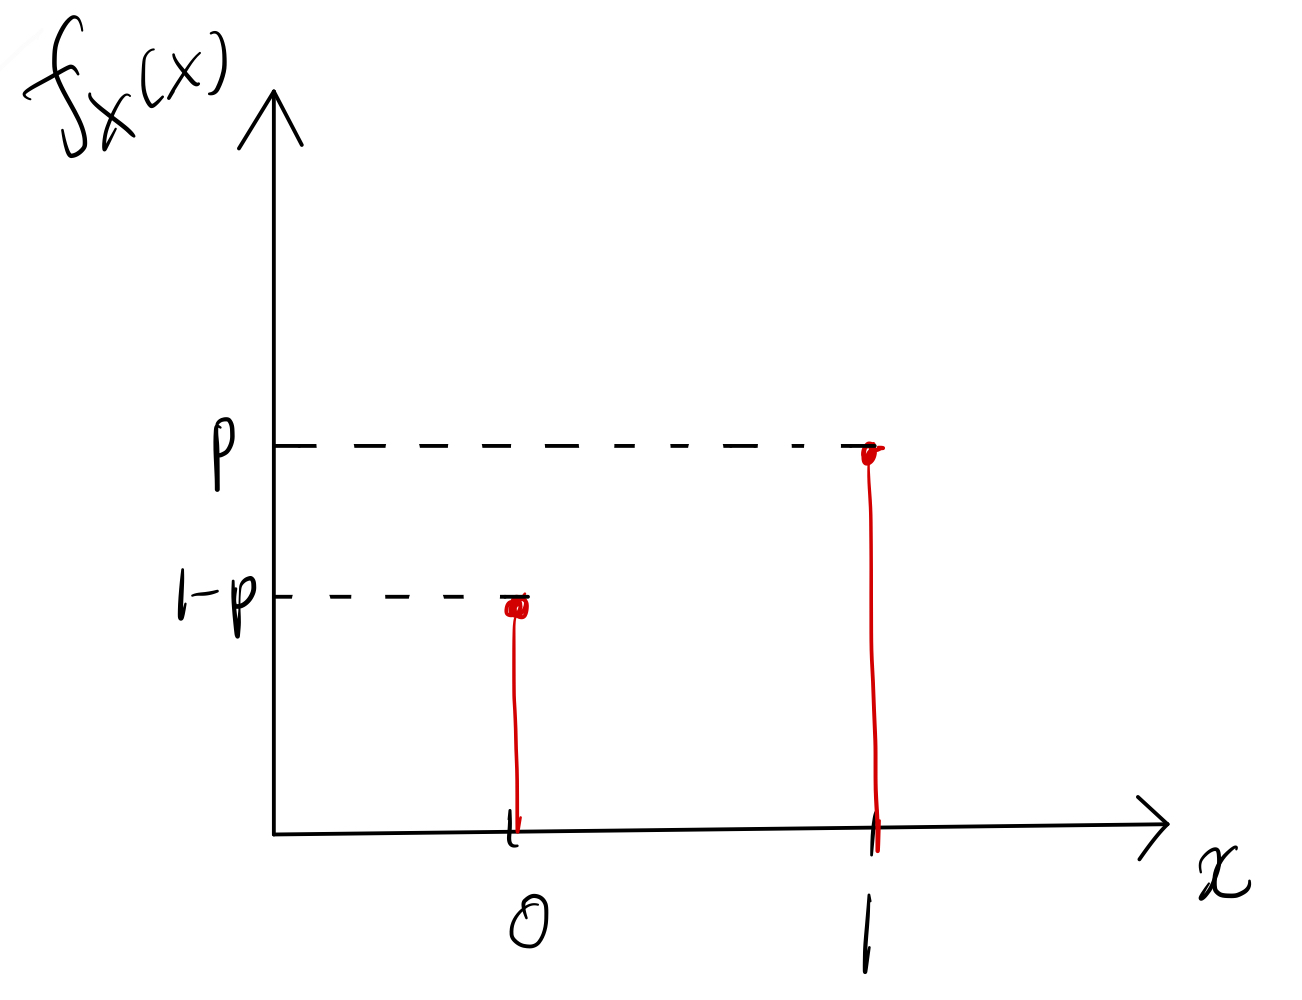
\includegraphics[width=0.5\textwidth]{figures/03-Probability_distribution/Bernoulli.jpeg}
      \caption{白努利分佈的機率質量函數}
      \label{fig:bernoulli}
    \end{figure}
    
    白努利分布的命名來自於瑞士數學家 Jacob Bernoulli(1654-1705),是最簡單也最常用的的離散型機率分布。所有的二元變數,舉凡性別的男女、疾病發病與否、是否接受治療、收縮壓是否於140毫米汞柱以上,將有興趣的類別編碼為 1,另一個類別編碼為 0 後,其分布均可用白努利分布來描述,其中參數 $p$ 為類別為 $1$ 的機率。簡單計算白努利分布之期望值和變異數可得到期望值為 $p$,變異數為 $p(1-p)$。

    \begin{custom}{思考}
        我們知道變異數是分佈取值分散性的度量。根據這個想法,白努利分布的變異數應該在 $p$ 取值多少時為最小、$p$ 取值多少時為最大?剛剛我們算出分布的變異數為 $p(1-p)$,這個結果是否符合你的預測?
    \end{custom}

\subsection{二項式分布}
    我們剛剛提到的白努利分布對應到的是擲一次銅板並觀察是否為正面。如果我們擲了同一枚銅板多次,然後再計算正面的次數,對應到的就是\textit{二項式分佈} (binomial distribution)。假設我們擲了 3 次銅板,每次擲銅板時正面機會均為 0.8,那麼有 2 次正面的情況共有 3 種:第一、二次正面、第三次反面;第一、三次正面、第二次反面;第二、三次正面、第一次反面。情況的總數可以用高中的組合數來計算,也就是$C^3_2$或寫做$\binom{3}{2}$。每種情況都是兩次正面、一次反面,所以機率都是 $0.8^2 \cdot 0.2$。因此,總共出現 2 次正面的機率可以寫作 $\binom{3}{2} 0.8^2 \cdot 0.2 = 0.384$。按照上述的算法,如果我們把 $X$ 令為投擲 $n$ 次銅板,每次正面機會為 $p$ 時,出現正面次數的隨機變數,那麼 $X$ 的機率質量函數可寫為:
    \[f_X(x) = \binom{n}{x} p^x (1-p)^{n-x},\qquad x \in \{0,1,2,...,n\}\]
    此時我們稱隨機變數 $X$ 服從次數參數為 $n$,機率參數為 $p$ 的二項式分布,寫作
    \[X \sim Binomial(n,p)\]

    二項式分佈的偏度隨著機參數率 $p$ 的不同而可能為左偏、對稱或右偏。如圖\ref{fig:binomial}繪製的機率質量函數所示,當 $p<0.5$ 時,二項式分佈呈現右偏;當 $p>0.5$ 時,二項式分佈呈現左偏;當 $p=0.5$ 時,二項式分佈為左右對稱。
    \begin{figure}[htbp]
      \centering
      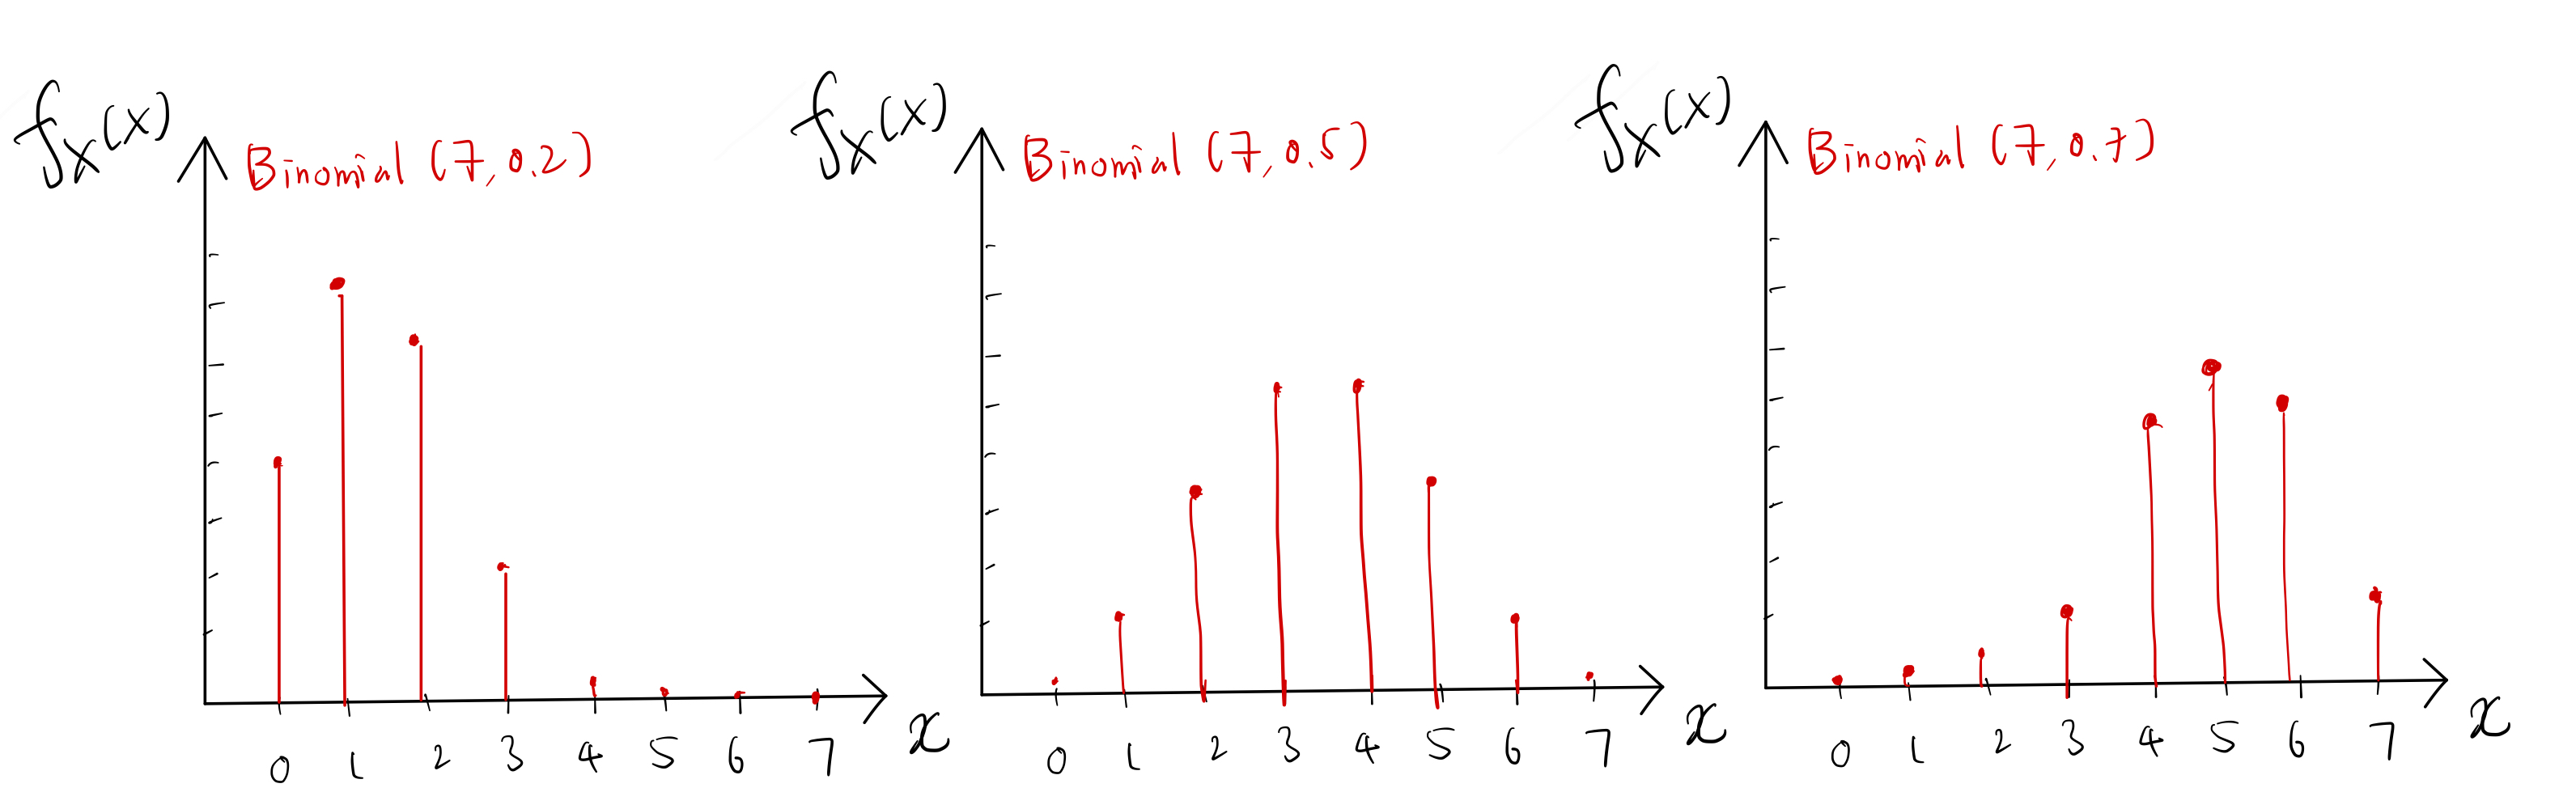
\includegraphics[width=\textwidth]{figures/03-Probability_distribution/Binomial.jpeg}
      \caption{二項分佈的機率質量函數}
      \label{fig:binomial}
    \end{figure}
    二項式分佈的期望值和變異數如果要從機率質量函數去推導,會需要相當麻煩的代數計算。但我們可以想像,二項式分佈所代表的銅板正面總次數,可以視為每次擲銅板時的正面次數(非 1 即 0)相加。如果 $X_1, X_2, ..., X_n$ 代表每次擲銅板正面與否,那麼他們都應該服從機率參數為 $p$ 的白努利分佈,而我們最終關心的正面總次數 $X = X_1 + X_2 + ... + X_n$。由於每次擲銅板的結果都是獨立的,所以根據我們前面提到有關期望值和變異數的性質:
    \begin{align*}
        \EE(X) &= \EE(X_1 + X_2 + ... + X_n)&\\
        &= \EE(X_1) + \EE(X_2) + ... + \EE(X_n) &\text{(相加的期望值等於期望值相加)}\\
        &= p + p + ... + p&\text{(每次擲銅板都服從} Bernoulli(p)\text{)}\\
        &= np&\\
        var(X) &= var(X_1 + X_2 + ... + X_n)&\\
        &= var(X_1) + var(X_2) + ... + var(X_n) &\text{(獨立隨機變數相加的變異數等於變異數相加}\\
        &= p(1-p) + p(1-p) + ... + p(1-p)&\text{(每次擲銅板都服從} Bernoulli(p)\text{)}\\
        &= np(1-p)&
    \end{align*}

    注意到這裡我們雖然是用擲銅板的正面次數來導出二項式分佈,但實際上二項式分佈可以用來描述一群樣本中,任意二元標籤的觀察總數。例如,如果抽樣 $n$ 位小細胞肺癌第三期的病患並統計三個月內復發的人數 $X$,那麼 $X$ 也會服從二項式分佈,其中次數參數為 $n$,機率參數 $p$ 則為「所有小細胞肺癌第三期的病患的三個月內復發機率」。
    
\subsection{卜瓦松分布}
    前面我們提到,如果我們有興趣的離散型隨機變數是二元的,可以用白努利分布描述;如果該離散型隨機變數可以被解釋為一群樣本中,二元標籤的觀察總數,則可以用二項式分布描述。但生物醫學中還有一種常見離散型資料:次數資料。這種離散型資料可以轉化為一段時間內事件發生的次數,例如三個月內的癲癇發作次數、每年嚴重藥物過敏的發生次數、胰臟癌每年新發個案等等。其可能取值為非負整數,最大可能取值為無上限、或可近似為無上限。

    \begin{figure}[htbp]
        \centering
        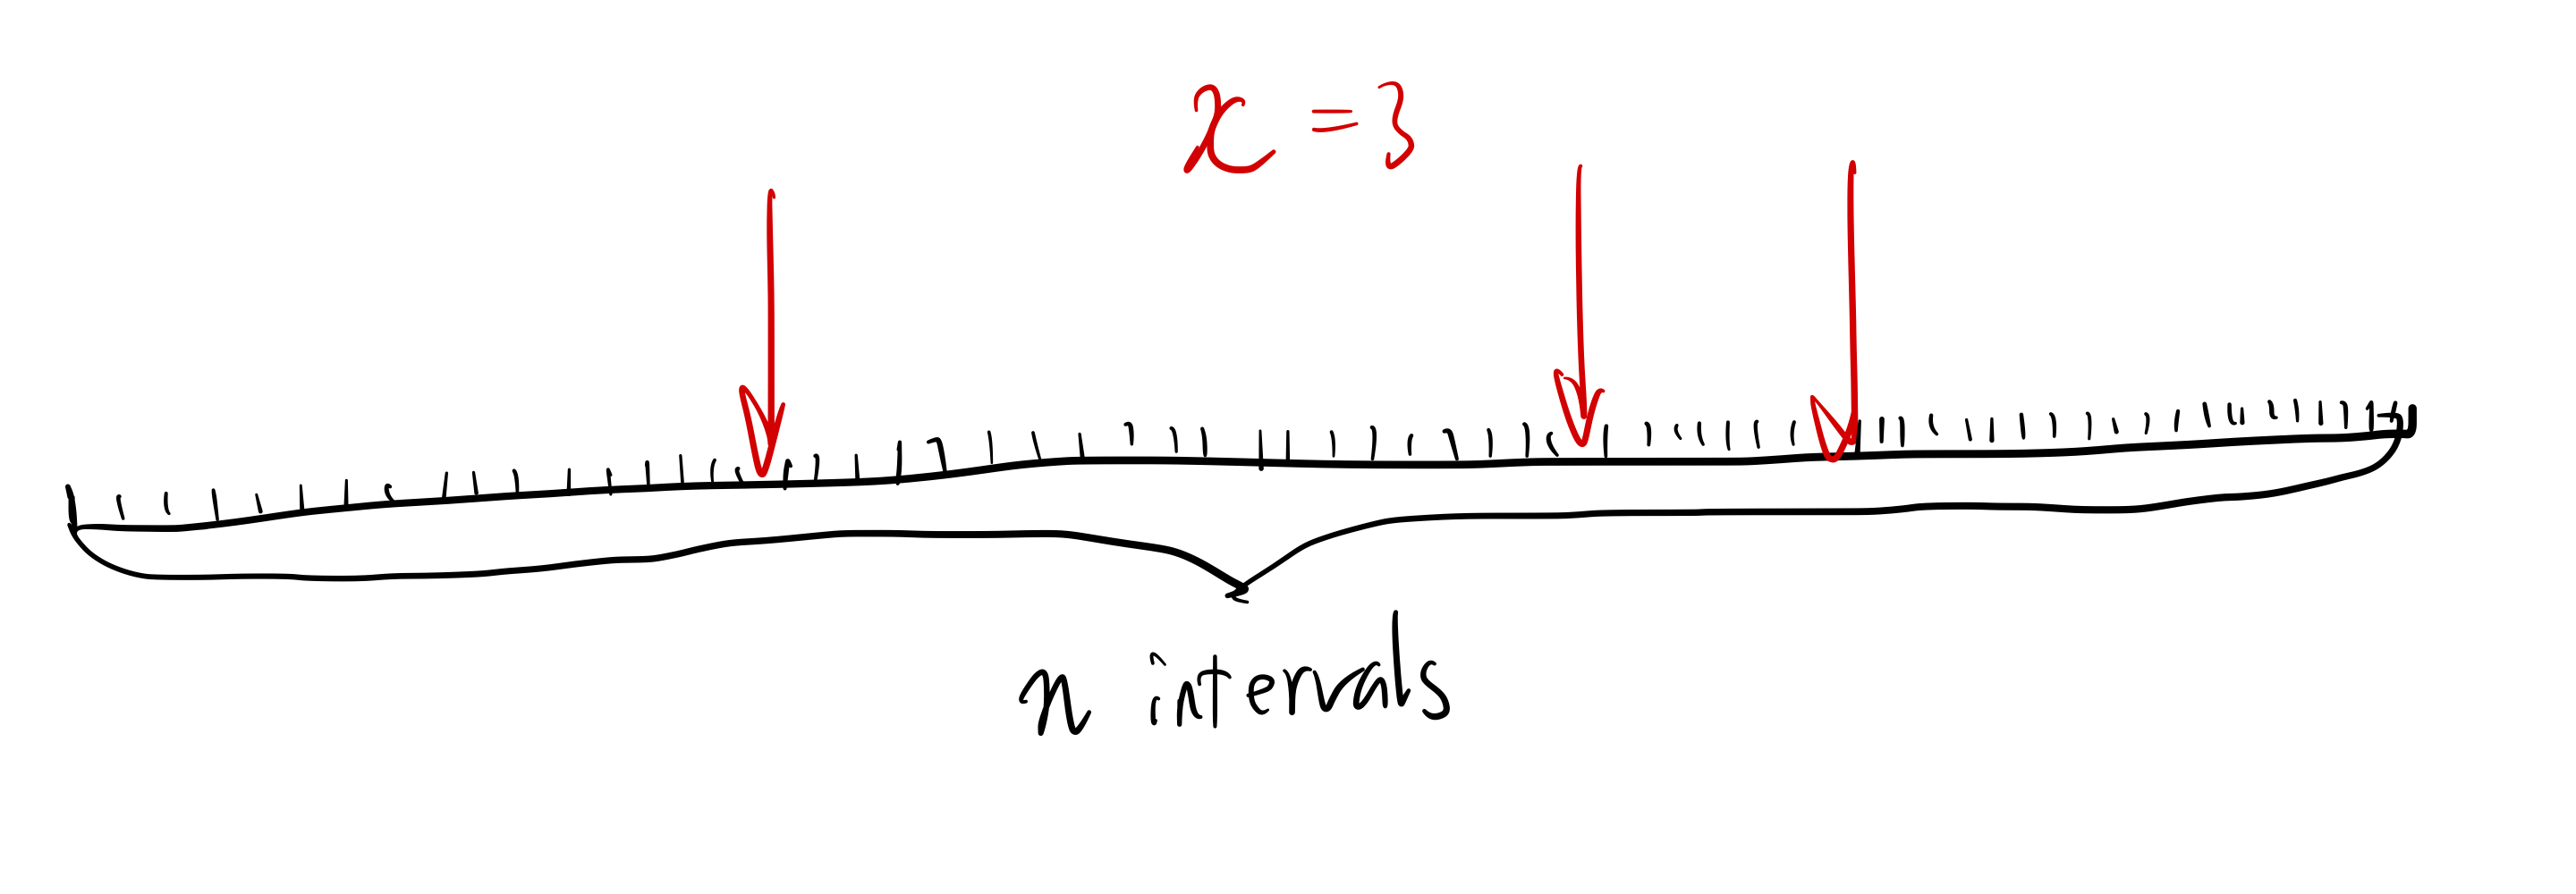
\includegraphics[width=0.7\textwidth]{figures/03-Probability_distribution/Poisson_exp.jpeg}
        \caption{以二項分布近似卜瓦松分佈}
        \label{fig:poisson_exp}
    \end{figure}

    描述次數資料最常用的分布是\textit{卜瓦松分布} (Poisson distribution),其命名來自於法國數學家 Siméon Poisson(1781-1840)。假設事件的發生滿足以下條件:(1) 發生事件之間為獨立 (2) 發生事件的頻率不隨時間點而改變 (3) 同一個時間點不會發生兩次以上的事件。那麼如圖\ref{fig:poisson_exp}所示,我們可以把追蹤的時間切成 $n$ 等分。根據上述的前兩個條件,每一等分發生事件的機率都相同且彼此獨立,而且在 $n$ 越來越大的情況下,根據第三個條件,每一個等分最多只會發生一件事件,且發生事件的機率可寫為 $\lambda/n$,其中 $\lambda$ 為在整段時間內預期發生事件的次數。整條時間線可以被看成作了 $n$ 次互相獨立、成功機率為 $\lambda/n$ 的實驗,而我們關心的是成功的總次數 $X$。在這個近似的框架下,$X$ 應該服從二項式分配,其機率質量函數可寫做
    \begin{align*}
        f_X(x) = \binom{n}{x} \Big(\frac{\lambda}{n}\Big)^x\Big(1-\frac{\lambda}{n}\Big)^{n-x} &= \frac{n (n-1)...(n-x+1)}{x!}\frac{\lambda^x}{n^x}\Big(1-\frac{\lambda}{n}\Big)^n\Big(1-\frac{\lambda}{n}\Big)^{-x}\\
        &= \frac{n (n-1)...(n-x+1)}{n^x} \Big(1-\frac{\lambda}{n}\Big)^{-x} \frac{\lambda^x}{x!} \Big(1-\frac{\lambda}{n}\Big)^n
    \end{align*}
    當切的等分數 $n$ 趨近於無窮大時,前兩項都會趨近於 $1$,而最後一項則會趨近於 $e^{-\lambda}$($e$是自然對數的底,約 2.718)。因此,卜瓦松分佈的機率質量函數為
    \[f_X(x) = \frac{\lambda^x e^{-\lambda}}{x!}, \qquad x \in \{0,1,2,3,...\}\]
    此時我們稱隨機變數 $X$ 服從速率參數 (rate parameter) $\lambda$ 的卜瓦松分布,寫作
    \[X \sim Poisson(\lambda)\]

    卜瓦松分布是一個右偏分布,如圖\ref{fig:poisson}所示,但偏度會隨著 $\lambda$ 增加而降低。根據前面用 $Binomial(n, \lambda/n)$ 二項式分佈的近似,卜瓦松分布的期望值為 $n \cdot (\lambda/n) = \lambda$。變異數則可用 $n \cdot (\lambda/n) \cdot (1- \lambda/n) = \lambda \cdot (1- \lambda/n)$ 近似,在 $n$ 趨近於無窮大時亦趨近至 $\lambda$。由此可知,卜瓦松分佈的特性為期望值和變異數相等。

    \begin{figure}[htbp]
        \centering
        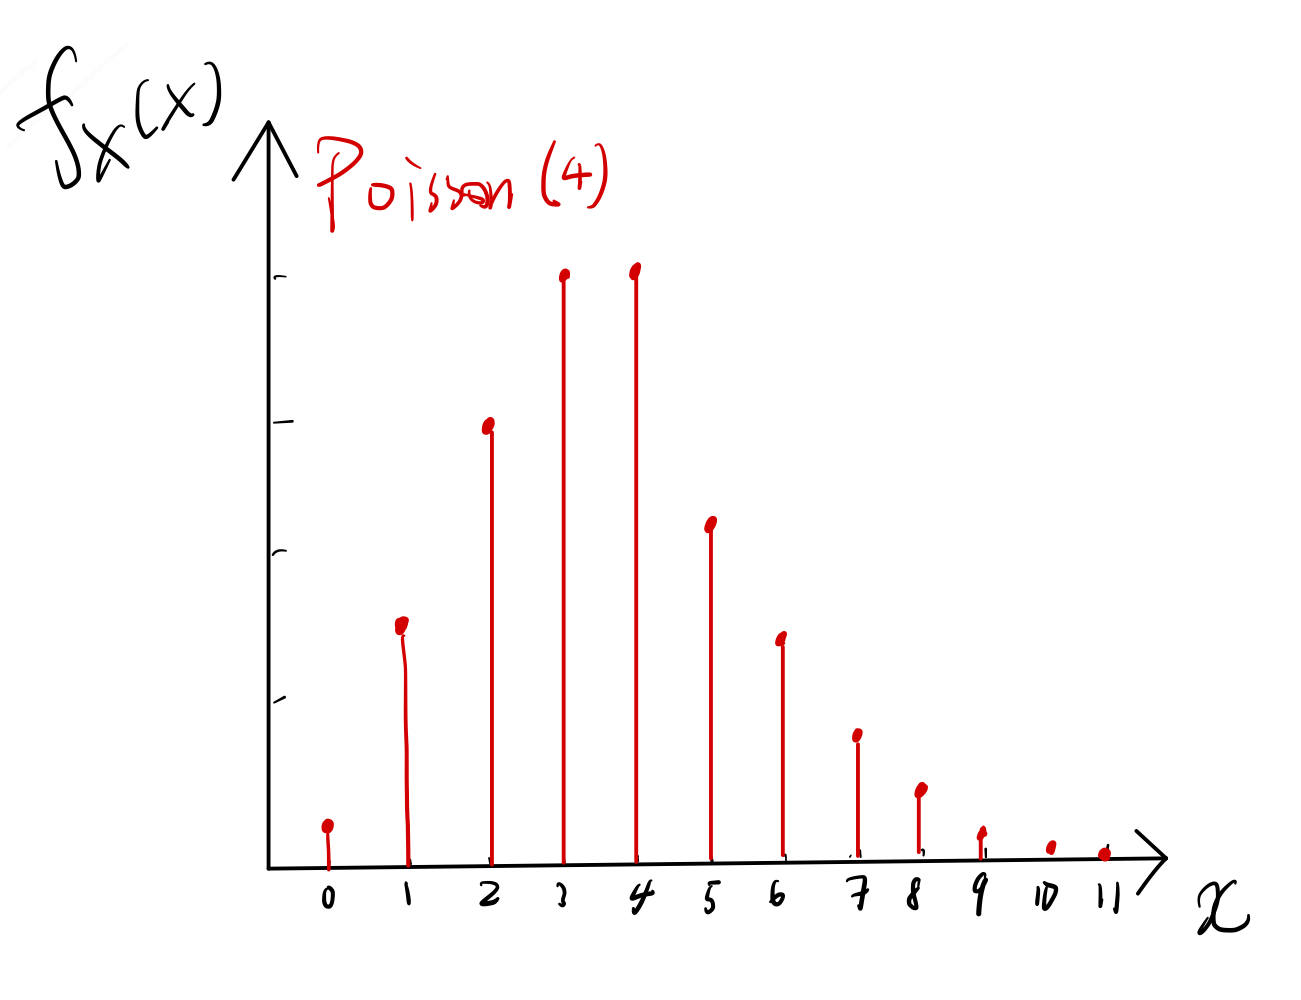
\includegraphics[width=0.6\textwidth]{figures/03-Probability_distribution/Poisson.jpeg}
        \caption{卜瓦松分佈的機率質量函數}
        \label{fig:poisson}
    \end{figure}

    \bigskip

    \begin{custom}{練習}
        根據一項大型世代研究,45 歲以上氣喘患者的平均急性發作率為一年 0.22 次。若氣喘發作的次數可用卜瓦松分配描述,那麼如何計算一位 45 歲以上氣喘患者在半年內發作兩次以上的機率?
    \end{custom}

    \bigskip

    \begin{custom}{思考}
        我們前面提到卜瓦松分佈的特性是期望值和變異數相等。如果我們抽樣的樣本並不「純粹」,而是來自多個速率參數不同的母體,那麼我們應該預期樣本變異數和樣本期望值的關係為何?
    \end{custom}

    \bigskip

    最後,我們用表\ref{tab:discrete_distribution}來總結生物醫學統計常用的離散型機率分布。
    
    \begin{table}[htbp]
        \begin{center}
            \begin{tabular}{cccc}
                \toprule
                分布名稱 & 參數 & 期望值 & 變異數\\
                \hline
                白努利 (Bernoulli) 分布 & 機率參數 $p$ & $p$ & $p(1-p)$\\
                二項式 (Binomial)分布 & 次數參數 $n$;機率參數 $p$ & $np$ & $np(1-p)$\\
                卜瓦松 (Poisson) 分布 & 速率參數 $\lambda$ & $\lambda$ & $\lambda$\\
                \bottomrule
            \end{tabular}
            \caption{生物醫學統計常用的離散型機率分布\label{tab:discrete_distribution}}
        \end{center}
    \end{table}
    
\section{連續型機率分布}

    前面我們提到,當隨機變數的可能取值可數(countable),就適合用離散型機率分布來描述,而且取得機率質量函數就完全決定了機率分布。然而,還有一類隨機變數的取值是連續而不可數的。舉例來說,如果我們在 Excel 裡輸入 \textit{RAND()} 函數,程式會隨機吐出一個 0 到 1 之間的亂數。我們把這個吐出的亂數記作隨機變數 $X$。如果小數位數無限增多,那麼從 0 到 1 之間的所有實數都是 $X$ 可能的取值,因此 $X$ 不是離散型的隨機變數,而是連續型的隨機變數,其所服從的也是一個\textit{連續型機率分布} (continuous probability distribution)。

    在連續型機率分布中,機率質量函數是沒有意義的。舉例而言,上述的 $X$ 若有機率質量函數 $f_X(x)$,則 $f_X(0.5)$ 應該代表 $X = 0.5$ 的機率。然而,$X$ 的取值是連續的,所以雖然 $X$ 可以取值 0.5,但 $X = 0.5$ 的機率等於零。事實上,$X$ 等於任何一個數的機率都等於零,所以 $X$ 的機率質量函數無法提供任何資訊。取而代之的是\textit{機率密度函數} (probability density function),如圖\ref{fig:uniform}所示。機率密度函數\textbf{曲線下的面積}代表取值區間出現的機率,例如圖中藍色的曲線下面積等於 $(0.7-0.4) \times 1 = 0.3$,代表 $X$ 取值於 0.4 到 0.7 之間的機率 $\PP(0.4 \le X \le 0.7) = 0.3$。我們也可以看到,如果區間取 「0.5 到 0.5 之間」,那麼曲線下就沒有面積,也就隱含著 $\PP(0.5 \le X \le 0.5) = \PP(X=0.5) = 0$,和我們前述單點機率等於零的結論相符。由於曲線下的面積才是機率,機率密度函數的實際取值並非機率而是\textit{機率密度} (probability density),用來度量隨機變數。也因此,雖然機率質量函數的取值不能超過 1(否則會違反總機率等於一的規則),但機率密度函數的取值卻可以超過 1,只要任何曲線下面積都不超過 1 即可。總機率等於一的規則在機率密度函數的體現,就是曲線下的總面積要等於一,寫成數學式就必須要動用到積分:
    \[\int_{-\infty}^{\infty} f_X(x) dx = 1\]
    讀者可以依此來檢查圖\ref{fig:uniform}的機率密度函數是否有符合總機率等於一的規則。
    \begin{figure}[htbp]
        \centering
        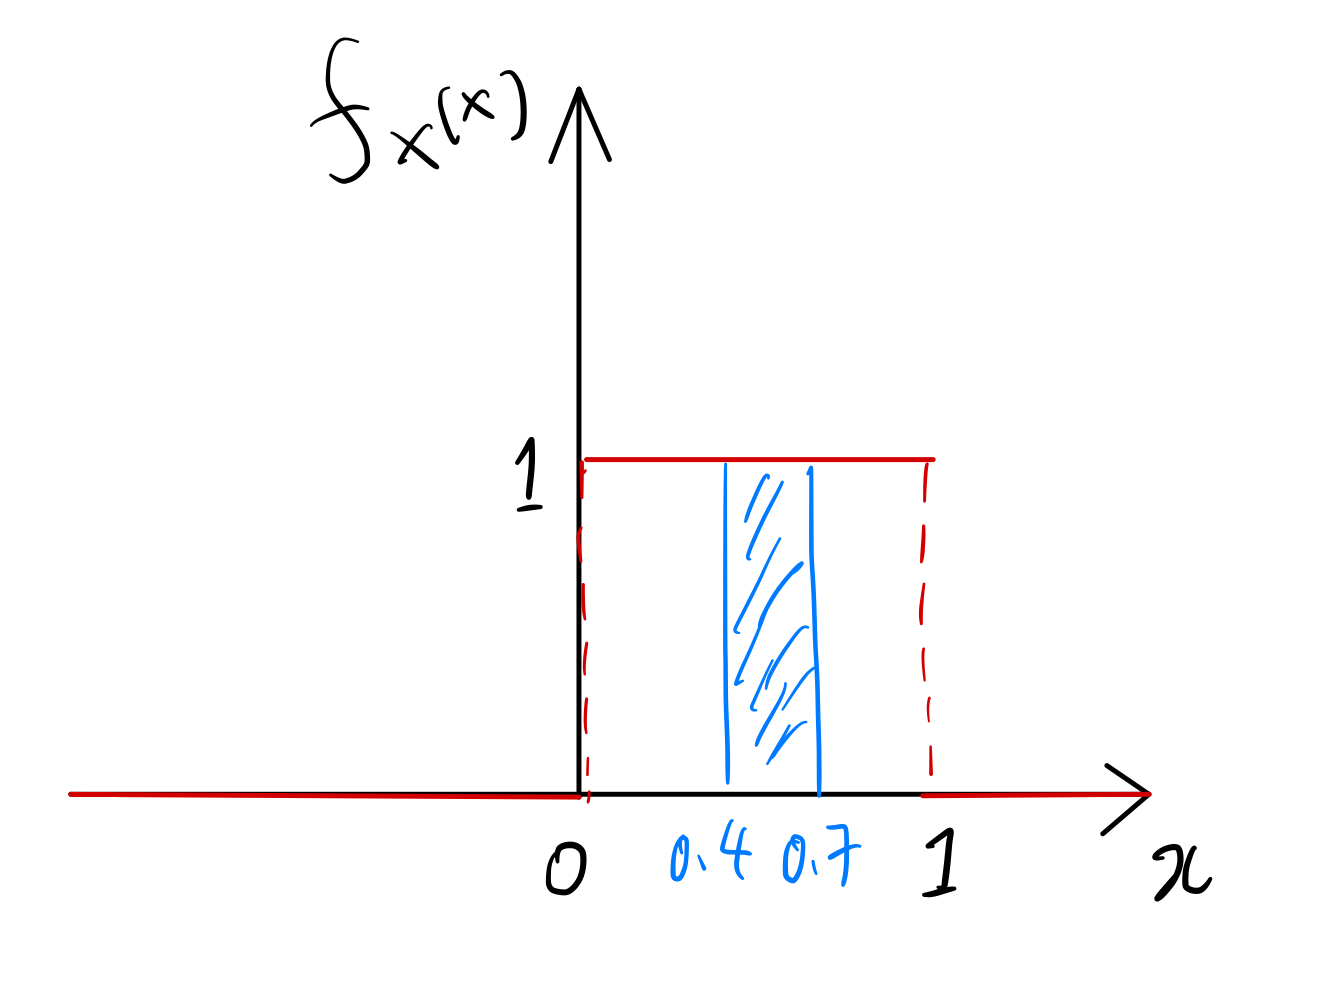
\includegraphics[width=0.6\textwidth]{figures/03-Probability_distribution/Uniform.jpeg}
        \caption{標準均一分布的機率密度函數}
        \label{fig:uniform}
    \end{figure}

    在離散型機率分布中,我們提到期望值的算法是將各取值以出現機率作加權平均,而變異數則是將「各取值與期望值距離的平方」以出現機率作加權平均。在連續型機率分布中,由於取值是連續的,我們需要將前面的定義用積分作小小的修正:
    \[\EE(X) = \int_{-\infty}^{\infty} x f_X(x) dx\]
    \[var(X) = \int_{-\infty}^{\infty} (x-\EE(X))^2 f_X(x) dx\]
    如果想要用 $var(X) = \EE(X^2) - (\EE(X))^2$ 來計算變異數,則需要用到
    \[\EE(X^2) = \int_{-\infty}^{\infty} x^2 f_X(x) dx\]

    另外,我們在離散型機率分布中提到的累積分配函數,在連續型機率分佈中仍然適用。其計算方式仍然需要用到積分:
    \[F_X(x) = \PP(X \le x) = \int_{-\infty}^x f_X(x) dx\]
    其中因為需要算出 $X \le x$ 的機率,也就是 $X$ 介於 $-\infty$ 和 $x$ 的機率,所以計算曲線下面積的積分上下限即為 $-\infty$ 到 $x$。
    
\subsection{常態分布}

    前面提到 0 到 1 之前的隨機亂數分布被稱為標準均一分布 (standard uniform distribution)。雖然標準均一分布在解釋上非常直覺,但實際上統計上最常用到的連續型分布是如圖\ref{fig:normal}左方的\textit{常態分布} (normal distribution)。常態分布又被稱為\textit{正態分布}或\textit{高斯分佈} (Gaussian distribution)。它有兩個十分直覺的參數:代表平均值的 $\mu$ 和代表變異數的 $\sigma^2$,其機率密度函數如下:
    \[f_X(x)=\frac{1}{\sqrt{2\pi\sigma^2}}e^{-\frac{(x-\mu)^2}{2\sigma^2}}\]
    當$\mu$的取值由高而低變動時,常態分布的曲線就會由右往左平移;當$\sigma^2$的取值由高而低變動時,常態分布的曲線就會由胖變瘦。此時我們稱 $X$ 服從平均值為 $\mu$、變異數為 $\sigma^2$ 的常態分布,記作
    \[X \sim Normal(\mu, \sigma^2) \qquad \text{或} \qquad X \sim \NN(\mu, \sigma^2)\]
    
    常態分布的機率密度函數雖然長得很醜陋,但常態分布是最能描述一般連續型隨機變數的分布,例如身高、體重、智商等等。從圖\ref{fig:normal}來看,常態分佈有一些重要的特徵:
    \begin{itemize}
        \item 單峰 (unimodal):常態分布最有可能取值在平均值 $\mu$ 附近。
        \item 對稱 (symmetric):常態分布以平均值 $\mu$ 為中心,左右對稱。因此,常態分布的中位數亦為 $\mu$。
        \item 鐘型 (bell-shaped):常態分佈在取值遠離平均值後,機率密度瞬間降低。事實上,我們在敘述性統計提到的經驗法則,就是由常態分布而來:常態分布取值在 $\mu \pm \sigma$ 之間的機率為 $68.2\%$;在 $\mu \pm 2\sigma$ 之間的機率為 $95.4\%$;在 $\mu \pm 3\sigma$ 之間的機率為 $99.7\%$。
    \end{itemize}

    \begin{figure}[htbp]
        \centering
        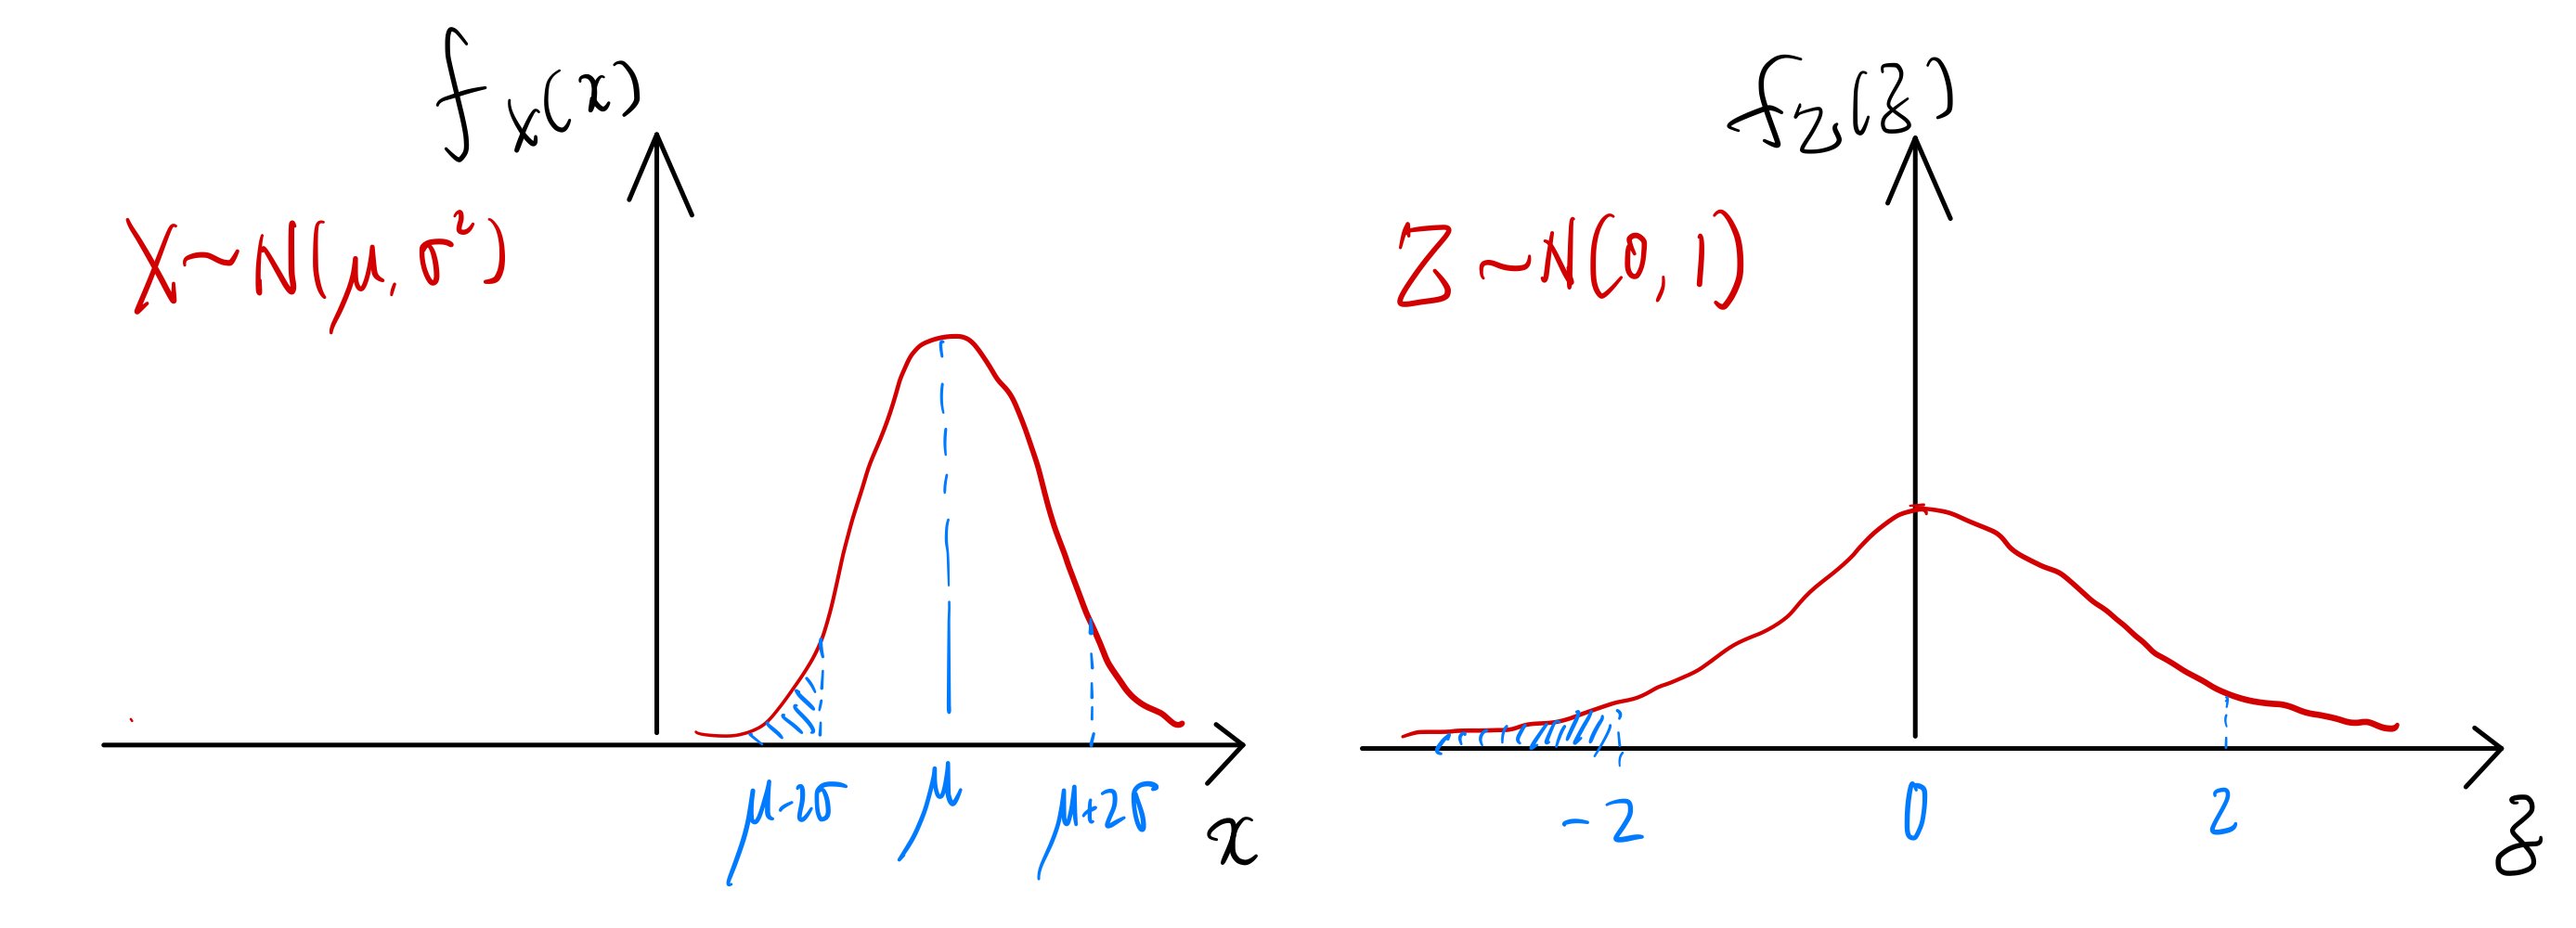
\includegraphics[width=\textwidth]{figures/03-Probability_distribution/Normal.jpeg}
        \caption{常態分布(左)與標準常態分布(右)的機率密度函數}
        \label{fig:normal}
    \end{figure}

    在所有的常態分布中,我們稱平均值$\mu =0$、變異數 $\sigma^2 = 1$的常態分布為\textit{標準常態分布} (standard normal distribution),如圖\ref{fig:normal}右方所示。其對應的隨機變數通常記為 $\ZZ$,機率密度函數則記為
    \[\phi(x)=\frac{1}{\sqrt{2\pi}}e^{-\frac{x^2}{2}}\]
    更重要的是,標準常態分布的累積分配函數常記為
    \[\Phi(x)=\int_{-\infty}^x \frac{1}{\sqrt{2\pi}}e^{-\frac{x^2}{2}} dx\]
    這個積分式只能用數值方法求值,但因為它十分重要,所以一般都會為這個函數製表,被稱為\href{https://en.wikipedia.org/wiki/Standard_normal_table}{標準常態表} (standard normal table) 或 Z 表 (Z table)。例如我們想知道 $\ZZ \ge 1.96$ 的機率,則因為常態分布是對稱的,$\ZZ \ge 1.96$ 的機率就等於 $\ZZ \le -1.96$ 的機率,查表得 $0.02500$。
    
    任何常態分布的隨機變數在經過 \textit{z轉換} (z-transform) 後都會變成標準常態分布。若 $X \sim \NN(\mu, \sigma^2)$,則
    \[\frac{X-\mu}{\sigma} \sim \NN(0,1)\]
    因此,任何常態分布的曲線下面積也都可以藉由 z 轉換求得:如果我們想知道 $X \ge x$ 的機率,那麼我們可以先算出 $x$ 經過 z 轉換後得到的 \textit{z 分數} (z-score):
    \[z = \frac{x-\mu}{\sigma}\]
    此時,我們有
    \[\PP(X \ge x) = \PP\Big(\frac{X-\mu}{\sigma} \ge \frac{x-\mu}{\sigma}\Big) = \PP(\ZZ \ge z)\]
    所以只要在標準常態表中查詢 $\ZZ \ge z$ 的機率即可。
    
    同樣的流程可以反過來做:如果我們想知道 $X$ 取值多少以上的機率為 $\alpha$,那麼我們可以先找出 $\ZZ$ 取值多少以上的機率為 $\alpha$(一般會把這個值記為 $z_\alpha$),然後我們就有:
    \[\alpha = \PP(\ZZ \ge z_\alpha) = \PP\Big(\frac{X-\mu}{\sigma} \ge z_\alpha \Big) = \PP(X \ge \mu + \sigma z_\alpha)\]
    亦即,只要把 $z_\alpha$ 視為 z 分數做反轉換,就可以找到欲求的取值閾值。
    
    \bigskip

    \begin{custom}{練習}
        假設已知清華大學的大學生身高服從一個平均值為 165 公分,標準差為 7 公分的常態分布。那麼我們預期會有多少比例的大學生身高介於 161.5 到 172 公分之間?如果我們想找出身高前 $1.5\%$ 的大學生,應該召集身高高於多少公分的學生?
    \end{custom}

    \bigskip

    \begin{custom}{練習}
        根據 WHO 定義,個人之骨質密度 T 分數 (T-score)為其骨質密度依 30-39 歲女性之骨質密度平均值與標準差作 z 轉換後所得之值。T 分數等於或低於 -2.5 者可被診斷為骨質疏鬆。假定台灣 30-39 歲女性股骨頸骨質密度之平均值及標準差為 $0.93 \pm 0.08$ g/cm$^2$、60-69 歲女性股骨頸骨質密度之平均值及標準差為 $0.76 \pm 0.15$ g/cm$^2$。若假定女性股骨頸骨質密度之分布遵從常態分布,則理論上台灣 60-69 歲女性中,有多少比例可因股骨頸骨質密度被診斷為骨質疏鬆?
    \end{custom}

    \begin{docexam}{(104-1醫學(一))}
        若已知國內男性抽菸盛行率為 $20\%$,隨機抽三位男性,三位都抽菸的機率為何?
    \end{docexam}

    \begin{docexam}{(102-1醫學(一))}
        某學生想為他這學期體育課的選課做出決定。假設一學期可選兩種運動課程,但選課人數一經額滿就無法選上。若此生選上游泳課的機率為 0.6,選上韻律課的機率為 0.5,同時選上游泳課和韻律課的機率為 0.3。此生選上韻律課或游泳課或兩種課程的機率為多少?
    \end{docexam}

    \begin{docexam}{(100-1醫學(一))}
        如果白人小孩的平均血漿醛固酮 (plasma-aldosterone) 為400 pmol/L,標準差為200 pmol/L,假設血漿醛固酮為常態分布,有多少百分比的白人小孩其血漿醛固酮$\le$ 300 pmol/L($Pr(\ZZ \ge 0.5) = 0.3085$)?
    \end{docexam}

    \begin{docexam}{(109-2醫學(二))}
        假設有一個疾病為顯性遺傳病,得病者父母親中,其中有一位有病,另一位則無。這種疾病每位子女遺傳的機率 $1/2$,一個有 2 個小孩的家庭,兩個小孩皆得病的機率為何?
    \end{docexam}